\section{Virtualised Network Functions in \headershortacr{3G} Core Networks}\label{sec:cloud:virtualized_network_functions}
\newcommand{\blockingprobability}[0]{p_B}
\newcommand{\maxServers}[0]{S_{\max}}
In this section we apply the theoretical methods discussed in \refsec{sec:cloud:data_centers} and apply them to the real-world challenge of virtualised network functions.
We consider the exemplary use case of a virtualised \gls{GGSN}.
Here, network operators consider the virtualisation of previously physical middleboxes, in order to gain elasticity and reduce costs.

In contrast to the last section, we assume a loss model, as connection establishment requests are not queued in reality but expire if no capacity is available.
Thus, we consider the blocking probability instead of the mean waiting time as a metric.
As a second metric we consider the number of provisioned servers which need to kept powered on. 

This section is structured as follows:
In \refsec{sec:cloud:virtualized_network_functions:model} we first introduce a model for a traditional \gls{GGSN}.
Then, we extend it to be applicable for the study of a virtualised \gls{GGSN}.
In \refsec{sec:cloud:virtualized_network_functions:measurement_data} we describe the procedures used to obtain and process input parameters for use in our simulation study.
Finally, in \refsec{sec:cloud:virtualized_network_functions:performance_evaluation} we study possible gains by a virtualised \gls{GGSN} by considering the tradeoff between the required servers to be active simultaneously and the incurred blocking probability. 

\subsection{Models of \headershortacr{GGSN} Implementations}\label{sec:cloud:virtualized_network_functions:model}

In this section we provide a model for a traditional \gls{GGSN} and discuss a model for a virtual \gls{GGSN} using \gls{NFV}.
In \gls{NFV} \cite{Nfv2013} static network middleboxes are replaced by commodity hardware.
The tasks solved by the original middleboxes are then solved by dedicated software.

\subsubsection*{Traditional GGSN}\label{sec:cloud:virtualized_network_functions:model:traditional_ggsn}
First, we give a model for a \emph{traditional} \gls{GGSN}, i.e. a static network component.
While we consider the \gls{GGSN} to be one fixed entity, it can in reality consist of multiple servers.
However, due to the fact that the \gls{GGSN} is purchased from a vendor as a middlebox, idle servers can be neither deactivated nor reused for other purposes.

\begin{figure}
  \centering
  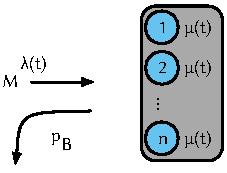
\includegraphics{cloud/virtualized_network_functions/model/figures/traditional_ggsn}
  \caption{Considered model of a traditional \headershortacr{GGSN}.}
  \label{sec:cloud:virtualized_network_functions:model:traditional_ggsn:model}
\end{figure}

We present an abstract queueing model for the traditional \gls{GGSN} in \reffig{sec:cloud:virtualized_network_functions:model:traditional_ggsn:model}.
New tunnels requests arrive according to a Poisson process with rate \(\lambda(t)\) at the \gls{GGSN}.
This server will support a maximum tunnel capacity of \(c\).
When this capacity is reached, blocking will occur and newly incoming tunnels requests are rejected.
Traditionally, \glspl{GGSN} can be expected to be overdimensioned in such a way that this rarely happens.
If the new tunnel is accepted, it will occupy one of the serving units of the server for the duration \(\mu(t)\) of the tunnel.
As stated earlier, we can not model the tunnel duration to be markovian, resulting in a  \(M/GI/c\) loss system.
In order to give quality of service guarantees the network operator is interested in the system's blocking probability \(\blockingprobability\), which we consider to be a key metric of our model.
Additionally, the previously described diurnal patterns can also be modelled by adjusting the arrival and serving process distributions for each time of day.
This alternatively also allows just to investigate the busy hour and thus the system's peak load.

\subsubsection*{\headershortacr{GGSN} using Network Function Virtualisation}\label{sec:cloud:virtualized_network_functions:model:virtual_ggsn}
Next, we introduce concepts from \gls{NFV}, i.e. the idea to replace middleboxes with commodity hardware as an extended model in \reffig{sec:cloud:virtualized_network_functions:model:virtual_ggsn:model}.
This allows us to realise benefits from cloud computing, as we are now able to scale out, instead of up.
The assumptions of the Markov arrival process \(\lambda(t)\) and the serving time distributions \(\mu(t)\) are carried over.
However, instead of one server processing every tunnel, this model assumes that there are up to \(s_{max}\) virtualised servers \(s_i\).
Each of these is less powerful than the traditional \gls{GGSN}, having a tunnel serving capacity of \(c_i \ll c\) and a total system capacity of \(c_{max} = s_{max} \times i\).

\begin{figure}
  \centering
  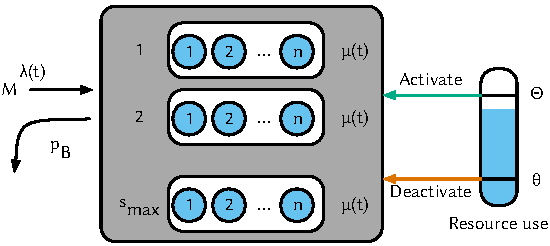
\includegraphics{cloud/virtualized_network_functions/model/figures/virtual_ggsn}
  \caption{Considered model of a virtualised \headershortacr{GGSN}.}
  \label{sec:cloud:virtualized_network_functions:model:virtual_ggsn:model}
\end{figure}

In its initial state, for efficiency, all but a small portion of the server instances are considered to be disabled.
Only, when a certain condition is reached, a new server instance is provisioned.
As a simple example, one instance could be kept in reserve for upcoming requests and an additional would be provisioned as soon as the reserve is used.
Similar rules should apply in the shut-down of servers and form a hysteresis with the boot condition.
For example it would be possible to keep at least one server in reserve but never more than two.

If these conditions are not carefully selected and are in tune with the expected boot time of an instance, additional blocking can occur.
Despite not having reached its maximum capacity, this system would still reject tunnel requests during the provisioning phase when no tunnel slots are available.
This could be remedied by a request queue.
However, this would introduce additional complexity to the system without providing real benefit, as mobile devices or applications will repeat their attempts and would timeout when the request is taking too long.

To place incoming tunnel state on one of the available servers a load balancer is required.
To ensure that the system in run time can scale down to its actual needs, the balancer should place tunnels on servers that are the fullest, keeping the reserve free.
It may even migrate tunnel state from almost empty servers away so that these can be shut down, when the shut-down condition is fulfilled.
Keeping instance close to their capacity should also have no impact on the performance a mobile device associated to a specific tunnel experiences.

\subsection{Measurement Data}\label{sec:cloud:virtualized_network_functions:measurement_data}

In order to evaluate our models introduced in \refsec{sec:cloud:virtualized_network_functions:model}, we use data gathered from a nation-wide mobile operator.
This allows for precise core network evaluations and the creation statistical fits for the observed processes.
In this section we first describe the dataset used for the evaluation and afterwards we derive the random variables required for our models.

\subsubsection*{Dataset Description}\label{sec:cloud:virtualized_network_functions:measurement_data:description}

\label{sec:dataset_description}

All data was collected by the \gls{METAWIN} monitoring system~\cite{Ricciato2006} with measurement probes located at the Gn interface within the core network, enabling broad access to signaling.
For this investigation we employ \gls{GTP} protocol data gathered by \gls{METAWIN}.
This data includes the \gls{RAT} identifier as well as the terminal types of the mobile clients, by use of the \gls{TAC} part of the \gls{IMEI}.
To meet privacy requirements, \gls{METAWIN} anonymizes all captured data.
The application-level payload is removed and all user identifiers are hashed with one-way functions before data storage.
Individual \glspl{UE} in our dataset can be differentiated by the hashed \gls{MS-ID}, but not traced back to the actual user.

The used dataset is a week-long trace from the third week of April 2011.
It consists of \(2.2\) billion aggregated flows for user traffic and \(410\) million \gls{GTP} Tunnel Management transactions.
It was tapped at one of the \glspl{GGSN} of the operator and contains about half of the total traffic volume handled by the operator in this period.

\subsubsection*{Statistical Evaluation}\label{sec:cloud:virtualized_network_functions:measurement_data:evaluation}

Using this dataset, we can obtain the distributions required for the models introduced in \refsec{sec:cloud:virtualized_network_functions:model}.
First, we study the tunnel interarrival time in \reffig{fig:cloud:virtualized_network_functions:measurement_data:evaluation:tunnel_iat}.

\begin{figure}
  \centering
  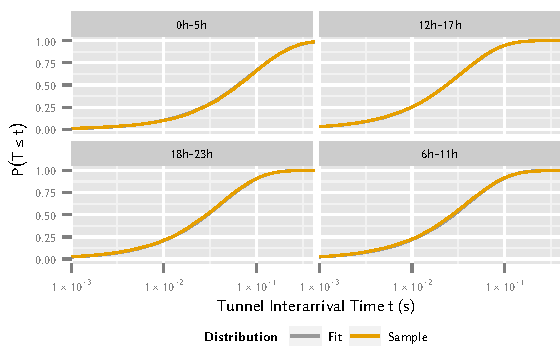
\includegraphics{cloud/virtualized_network_functions/measurement_data/figures/tunnel_iat}
  \caption{Empirical and exponentially fitted CDFs of the tunnel interarrival duration by time of day. CDFs are overlapping as the coefficient of determination is close to \(1\).}
  \label{fig:cloud:virtualized_network_functions:measurement_data:evaluation:tunnel_iat}
\end{figure}

The arrival of new tunnel requests can be used as a measure for the load a \gls{GGSN} experiences, as every incoming tunnel carries several signaling interactions, processing and state with it.
Typically, a device will only hold one tunnel at a time, but this tunnel can be initiated and shut down in rapid succession, causing the aforementioned issues in the radio network.
The arrivals also show a strong diurnal effect, closely resembling patterns present in the actual user traffic:
We observe a decline of arrivals, i.e. longer interarrivals, late in the night and during the early morning hours with a peak rate in the afternoon and early evening.
To represent this time-of-day dependence in the model, the measurement was split into the four time slots displayed in the figure.
Each slot was then fitted with an exponential distribution by way of moment matching.
This results in the cumulative distribution function \(F(x) = 1- e^{-\lambda x}, x \geq 0\) with \(\lambda\) given in \reftab{tab:cloud:virtualized_network_functions:measurement_data:evaluation:iat_fits} for the four time slots.
The fitted functions match the empirical data, with some deviation present at the left tail but overall with a positive correlation coefficient approaching \(1\).

\begin{table}
  \centering
  \caption{Parameters for the exponentially distributed inter-arrival times and corresponding Pearson correlation coefficients}
  \label{tab:cloud:virtualized_network_functions:measurement_data:evaluation:iat_fits}  
  \begin{tabular}{ccc}
  \toprule
  Time of Day & \(\lambda\) & \(R_{arr}\)\\
  \midrule
  0h-5h & $10.67$ & $0.99$\\
  6h-11h & $24.53$ & $0.99$\\
  12h-17h & $29.25$ & $0.99$\\
  18h-23h & $23.49$ & $0.98$\\
   \bottomrule
  \end{tabular}
\end{table}

The second important tunnel property is the duration of the \gls{PDP} Context state accompanying a \gls{GTP} tunnel held at the \gls{GGSN}.
\reffig{fig:cloud:virtualized_network_functions:measurement_data:evaluation:tunnel_duration} shows the tunnel durations split up for the time of day, as there is once again a slight diurnal effect present, albeit with shifted peaks.
Longer tunnels tend to occur at night, shorter tunnels during midday.
Further properties of the tunnel duration, especially the correlation with device types and operating systems, are investigated in detail in~\cite{Metzger2014}.

\begin{figure}
  \centering
  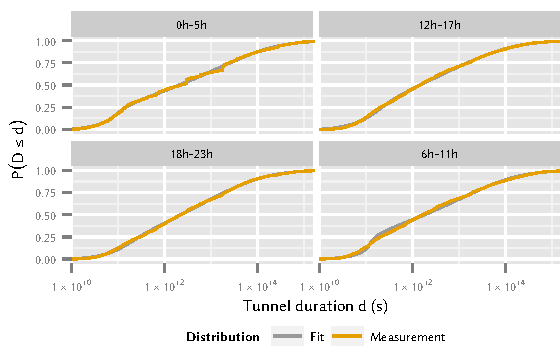
\includegraphics{cloud/virtualized_network_functions/measurement_data/figures/tunnel_duration}
  \caption{Empirical and fitted CDFs of the tunnel duration by time of day with fitted rational functions.}
  \label{fig:cloud:virtualized_network_functions:measurement_data:evaluation:tunnel_duration}
\end{figure}

\begin{table}
  \centering
  \caption{Inverse functions fitted to the empirical duration distribution and correlation coefficients of the fit.}
  \label{tab:cloud:virtualized_network_functions:measurement_data:evaluation:duration_fits}  
  \begin{tabular}{ccc}
  \toprule
  Time of Day & Inverse Fitted Duration Function & \(R_{dur}\)\\
  \midrule
  0h-5h & $0.91 - 60.61y - 3498.78y^3 - \frac{110.70y + 2289.94y^3}{y - 1.00}$ &  $0.99$ \\
  6h-11h & $1 + 117.48y - 368.64y^2 - \frac{1720.13y^4}{y - 1.00}$ & $0.99$ \\
  12h-17h & $0.95 + 69.49y + \frac{81146.10y^3 + 1.08\times10^6y^5}{805 - 802.01y}$ & $0.99$ \\
  18h-23h & $0.91 + 82.05y - \frac{2936.93y^4}{1.94y - 1.95}$ & $0.99$\\
  \bottomrule
  \end{tabular}
\end{table}

Furthermore, the model requires information on the tunnel durations.
However, none of the basic probability distributions, e.g. exponential, gamma, and weibull distributions, fit the tunnel duration well enough.
One of the reasons for this probably being the correlation of the tunnel duration to a large number of factors, including user behavior and network-specific timers and procedures, e.g. tunnels are shut down by the network after specific events, introducing artifacts which make it hard to fit any distribution against.
Instead, we fit rational functions to the empirical \gls{CDF} using the Eureqa \cite{Schmidt2009} software.

This allowes for a much closer fit while still smoothing out some of the artifacts.
\reftab{tab:cloud:virtualized_network_functions:measurement_data:evaluation:duration_fits} displays these functions fitted to the inverse \gls{CDF}, to be directly used for generating random numbers using the inversion method.
Both the \gls{CDF} in \reffig{fig:cloud:virtualized_network_functions:measurement_data:evaluation:tunnel_duration} as well as the Pearson correlation coefficient confirm the goodness of the fitted functions.

\subsection{Inferring State Transitions and Deriving Metrics}\label{sec:network:network_traces:performance_evaluation}
A \gls{UE}’s firmware triggers \gls{RRC} state transitions based on application traffic.
While solutions exist to capture RRC state transitions on specific hardware~\cite{zayas2010} they are not available for all modern smartphone platforms.
Other options to measure the required information include using costly hardware and use specific \glspl{UE}, usually not available to researchers and application developers.
This prevents the developers from evaluating the effect of their applications on the overall health
of the network.
Consequently, they can not take measures to prevent the harmful behaviour of their applications.
However, it is possible to infer the \gls{RRC} state transitions for a given packet trace if the network configuration is known.

First, we describe the setup used to capture network packet traces for arbitrary apps.
Then, we give an algorithm to infer the \gls{RRC} state transitions for a given packet trace.
Based on these state transitions, we can calculate the number of signalling messages generated
by the packet trace. 
Finally, we use the information on when which \gls{RRC} state was entered to calculate the power drain of the \gls{UE}’s radio interface.

\subsubsection*{Measurement Procedure and Setup}\label{sec:network:network_traces:performance_evaluation:measurement}
To investigate the behaviour of the application under study, we capture traffic during a typical use of the application on a \emph{Samsung Galaxy SII} smartphone.
The smartphone runs the Android operating system and is connected to the \gls{3G} network of a major German network operator.
To obtain the network packet traces we use the \texttt{tcpdump} application.
This application requires \emph{root} privileges which are obtained by rooting the device and installing the custom \emph{cyanogenmod} ROM \footnote{\url{http://www.cyanogenmod.org}, Accessed: November, \(21^{st}\) 2015}.
Once \texttt{tcpdump} is installed and running, we start the application under study and capture packet traces while the application is running.
Then, the \emph{android debugging bridge} is used to copy the traces to a workstation.
The traces contain \gls{IP} packets embedded in Linux Cooked Captures.
We require the \gls{IP} packets, thus we extracted the \gls{IP} packets which are used during the analysis to follow.

\subsubsection*{Inferring Network State}\label{sec:network:network_traces:performance_evaluation:inferring_network_state}
In this section we study the influence of the application traffic on \gls{RRC} state transitions and signalling messages.
Since \gls{RRC} state transitions can not be captured using commonly available tools, we introduce an algorithm to infer \gls{RRC} state transitions from \gls{IP} packet traces.
Using this algorithm we analyse the \gls{RRC} state transition frequency and signalling message load for the Two State Model and Three State Model.

Traffic below the network layer can not be measured without specific equipment which interfaces with the proprietary firmware of the \gls{UE} and is often out of reach for developers interested in assessing the impact of their applications on the network.
Based on the Two State and Three State models introduced in \refsec{sec:network:background:umts_rrc}, we process \texttt{tcpdump} captures of the application traffic.
However, it should be noted that this method is not restricted to a specific network model, but can be extended to any other network model as well.
Using these captures, we extract the timestamps when \gls{IP} packets are sent or received.
Furthermore, we require the timer values of the transition from \gls{RRC_DCH} state to \gls{RRC_FACH} state, \gls{TDCH}, and the timer for the transition between \gls{RRC_FACH} and \gls{RRC_idle} states, \gls{TFACH}.
Based on these informations \refalg{alg:network:network_traces:performance_evaluation:inferring_network_state:inference_algorithm} infers the timestamps of state transitions according to the \gls{3GPP} specification \cite{3GPP_RRC_Spec} for the Three State Model.
This algorithm can be simplified to also work for the Two State Model. 
Alternatively, a method to post process the results of the algorithm to obtain results for the Two State Model is given at the end of this section.
The algorithm first computes the inter-arrival times of all packets.
Then, each timestamp is considered.
If the \gls{UE} is currently in \gls{RRC_idle} state, a state transition to \gls{RRC_DCH} occurs at the moment the packet is sent or received.
If the inter-arrival time exceeds the \gls{TDCH} timer the \gls{UE} transitions to \gls{RRC_FACH} \gls{TDCH} seconds after the packet was sent or received.
Similarly, if the inter-arrival time exceeds both the \gls{TDCH} and \gls{TFACH} timers a state transition to \gls{RRC_idle} occurs \gls{TDCH} seconds after the state transition to \gls{RRC_FACH}.

\begin{algorithm}
  \begin{algorithmic}
    \Require{Packet arrival timestamps \emph{ts}\\
    \gls{RRC_DCH} to \gls{RRC_FACH} timer \gls{TDCH}\\
    \gls{RRC_FACH} to \gls{RRC_idle} timer \gls{TFACH}}
    \Ensure{Times of state transition \emph{state\_time}\\
    New states after state transitions \emph{state}}
    \State \texttt{interarrival(i)} $\leftarrow$ \emph{ts}(i+1) - \emph{ts}(i)
    \State \texttt{index} $\leftarrow 0$
    \ForAll{ts(i)}
      \If{\texttt{state(index)} = \gls{RRC_idle}}
        \State \texttt{index} $\leftarrow$ \texttt{index} + 1
        \State \texttt{state(index)} $\leftarrow$ \gls{RRC_DCH}
        \State \texttt{state\_time(index)} $\leftarrow$ ts(i)
      \EndIf
      \If{\texttt{interarrival}(i-1) $> \gls{TDCH}$}
        \State \texttt{index} $\leftarrow$ \texttt{index} + 1
        \State \texttt{state(index)} $\leftarrow$ \gls{RRC_FACH}
        \State \texttt{state\_time(index)} $\leftarrow$ ts(i) $+ \gls{TDCH}$
      \EndIf
      \If{\texttt{interarrival}(i-1) $> \gls{TDCH} + \gls{TFACH}$}
        \State \texttt{index} $\leftarrow$ \texttt{index} + 1
        \State \texttt{state(index)} $\leftarrow$ \gls{RRC_idle}
        \State \texttt{state\_time(index)} $\leftarrow$ ts(i) $+ \gls{TDCH} + \gls{TFACH}$
      \EndIf
    \EndFor
  \end{algorithmic}
  \caption{Inferring \headershortacr{RRC} state transitions based on \headershortacr{IP} timestamps.}
  \label{alg:network:network_traces:performance_evaluation:inferring_network_state:inference_algorithm}
\end{algorithm}

Decreasing power drain of their devices is always a goal of \gls{UE} vendors.
A straightforward way to achieve this, if only the wellbeing of the \gls{UE} is considered, is to transition from \gls{RRC_DCH} state to \gls{RRC_idle} as soon as no additional data is ready for sending.
While this transition is not directly available in the 3GPP specification for the \gls{RRC} protocol \cite{3GPP_RRC_Spec}, a \gls{UE} may reset the connection, effectively transitioning from any state to \gls{RRC_idle}.
This behaviour can be modeled using the Two State Model introduced in \refsec{sec:network:background:umts_rrc}.

State transitions for the Two State Model can be calculated using a similar algorithm.
Alternatively, the behaviour of the Two State Model can be emulated using \refalg{alg:network:network_traces:performance_evaluation:inferring_network_state:inference_algorithm} if \gls{TFACH} is set to \SI{0}{\second} and all state transitions to \gls{RRC_FACH} are removed in a post processing step.

\subsubsection*{Calculating Signalling Frequency and Power Drain}\label{sec:network:network_traces:calculating_metrics}

\begin{table}
\centering
  \caption{Number of signalling messages per \headershortacr{RRC} state transition perceived at the \headershortacr{RNC} \cite{3GPP_RRC_Spec}.}
  \label{tab:network:network_traces:calculating_metrics:signalling_messages}
\begin{tabular}{lccc}
	\toprule
    from/to & \gls{RRC_idle} & \gls{RRC_FACH} & \gls{RRC_DCH}\\
    \midrule
    \gls{RRC_idle} & -- & 28 & 32\\
    \gls{RRC_FACH} & 22 & -- & 6\\
    \gls{RRC_DCH} & 25 & 5 & --\\
    \bottomrule    
	\end{tabular}
\end{table}

In reality, the number of state transitions is not the metric of most importance if network signalling is to be evaluated.
Each state transition results in a number of \gls{RRC} messages between the \gls{UE} and different network components.
For this study we consider the number of messages observed at the \gls{RNC}, which can be found in \cite{3GPP_RRC_Spec} and is summarized in \reftab{tab:network:network_traces:calculating_metrics:signalling_messages}.
It can be seen that transitions from or to the \gls{RRC_idle} state are especially expensive in terms of number of messages sent or received.
This is due to the fact that upon entering or leaving the \gls{RRC_idle} state, authentication has to be performed. 
Note that for the Two State Model only transitions from or to the \gls{RRC_idle} state occur.
This results in the fact that for the same network packet trace the number of signalling messages occurring in the Two State Model is generally higher than in the Three State Model.
To obtain the total number of signalling messages, we weight the number of state transitions with the number of messages sent per state transitions.
Then, we average the number of state transitions over the measurement duration to obtain a metric for the signalling load at the \gls{RNC}, i.e. the \gls{SF}.
The inference algorithm does not differentiate between state changes caused by upstream or downstream traffic.
State changes caused by downstream traffic usually generate some additional signalling messages, as paging is involved.
The inference algorithm can easily be enhanced to support this behaviour.
However, the results discussed in the next section would only change quantitatively.
Furthermore, the algorithm can be adapted to new networking models or other numbers of signalling messages sent per state transition.

\begin{table}
  \centering
  \caption{Power consumption of the \headershortacr{UE} radio interface depending on current \headershortacr{RRC} state \cite{Qian2011a}.}
  \label{tab:network:network_traces:calculating_metrics:power_consumption}  
  \begin{tabular}{lc}
  	\toprule
    \gls{RRC} State & Power Consumption\\
    \midrule
    \gls{RRC_idle} & \SI{0}{\milli\watt}\\
    \gls{RRC_FACH} & \SI{650}{\milli\watt}\\
    \gls{RRC_DCH} & \SI{800}{\milli\watt}\\
    \bottomrule
  \end{tabular}
\end{table}

From a users point of view, the signalling message frequency is of little importantance.
The user is interested in a low power drain as this increases the battery life of the device.
To calculate the battery life, we use the time when state transitions occurred, and the information about the state the transition was to, to calculate the relative amount of time that was spent in each state.
Given the relative time spent in each state, we use \reftab{tab:network:network_traces:calculating_metrics:power_consumption}, taken from \cite{Qian2011a}, to compute the \gls{PD} of the radio interface during the measurement phase.
We focus on the power drain of the radio interface, as it is possible to measure the aggregated power drain using out of the box instrumentation techniques provided by the hardware vendor.